\subsection*{Solution Design}
The first prototype will take inspiration from FTP streaming for file data transfer. Using UDP with this should reduce the total latency for a transfer; since all file data packets can be sent with no interruption for waiting for acknowledgments.

This prototype will use the binary protobuf format for structuring the packet data. This will reduce the amount of required overhead needed for storing structured data. Binary is suited for this prototype since it does not need to be easily human readable since only the software will be directly interacting with the data.

\subsubsection*{Packet Structure}
The packets structure will be split into several fields, using flexible offsets meaning the packet size is dynamic. Having a dynamic packet size should reduce the amount of wasted space, leaving more available space for the actual file data.

A packet will feature two protobuf fields one for the header which will describe what the packet is, and the second will include any extra metadata relevant to a request/response. The packets fields are illustrated in Table~\ref{tab:p1d-packet-fields}.

\begin{table}[h!]
    \caption{Prototype One Packet Fields}
    \label{tab:p1d-packet-fields}
    \centering
    \begin{tabular}{ l l l }
        \hline
        \textbf{Num} & \textbf{Name}   & \textbf{Data-Type} \\
        \hline
        001          & Type            & uint8              \\
        \hline
        002          & Header Length   & uint64             \\
        \hline
        003          & Header          & protobuf           \\
        \hline
        004          & Metadata Length & uint64             \\
        \hline
        005          & Metadata        & protobuf           \\
        \hline
        006          & Payload Length  & uint64             \\
        \hline
        007          & Payload         & binary             \\
        \hline
    \end{tabular}
\end{table}

The first field will take up exactly 1 byte, this field will be used to set the type of the packet. This will determine what protobuf encoded header structure will be. Using 1 byte will allow for 255 possible message types. Since these prototypes will not be a fully implemented solution only a few types will be implemented, which are shown in Table~\ref{tab:p1d-packet-types}.

\begin{table}[h!]
    \caption{Prototype One Packet Types}
    \label{tab:p1d-packet-types}
    \centering
    \begin{tabular}{ l l l }
        \hline
        \textbf{Prefix} & \textbf{Value} & \textbf{Note}                \\
        \hline
        SYN             & 1              & Perform connection handshake \\
        \hline
        ACK             & 2              & Acknowledge request          \\
        \hline
        REQ             & 3              & Request to send/receive      \\
        \hline
        PSH             & 4              & Send payload data            \\
        \hline
        FIN             & 254            & End connection               \\
        \hline
    \end{tabular}
\end{table}

The next field will take up 8 bytes, this will be big-endian ordered number which will say how many bytes of data to expect after for the header (an offset value).

After header length the actual header will follow, if there is no header the next field will immediately follow.

The 4th field will be the metadata length which is the same as the header length, however specifies the length of the metadata field.

The metadata field is the same as the header.

An example of a SYN packet in both a structured view and a hex representation of the binary data is shown in Listing~\ref{lst:p1d-example-structure} and Listing~\ref{lst:p1d-example-binary}.

\begin{minipage}{\textwidth}
    \begin{lstlisting}[caption={Prototype One Example Packet Structure},label=lst:p1d-example-structure]
|-------------------|
| 1                 | <- Packet Type
| 5                 | <- Header Length
| {id: 1, mtu: 470} | <- Protobuf Header (JSON representation)
| 0                 | <- No Metadata
| 0                 | <- No Payload
|-------------------|
\end{lstlisting}

    \begin{lstlisting}[caption={Prototype One Example Packet Binary},label=lst:p1d-example-binary]
 1 0 0 0 0 0 0 0 5 8 1 16 214 3 0 0 0 0 0 0 0 0 0 0 0 0 0 0 0 0
 ^ ^^^^^^^^^^^^^^^ ^^^^^^^^^^^^ ^^^^^^^^^^^^^^^ ^^^^^^^^^^^^^^^
 |        |             |              |               |
Type    Header        Header        Metadata        Payload
        Length                       Length         Length
\end{lstlisting}
\end{minipage}

\subsubsection*{Operation}
For a client to first connect to the server a simple handshake will occur. This has been based on the rsync protocol handshake which only requires one exchange at the start. The client will first send a packet type called "SYN" which includes the clients max receiving MTU size, this allows for the message size to be adjusted depending on the network structure. After the server has received it will acknowledge the handshake and send back it's own "SYN" packet, which will contain it's maximum supported receiving MTU and a generated client ID. This client ID will be stored at the server until the client disconnects, this will allow for a connection to remain available without the client needing to renegotiate. Because this ID will be used to determine which client is which, each message sent by the client will need this ID attached. Every message from the client following "SYN", must also increment a request ID field, which will allow error checking functionality.

\begin{itemize}
    \item Client: \url{https://github.com/enchant97/file-sync-protocol/blob/d0c709bd49d64598da03774df4ae5443802b8716/prototypes/proto-1/client.go#LL29C1-L46C42}
    \item Server: \url{https://github.com/enchant97/file-sync-protocol/blob/d0c709bd49d64598da03774df4ae5443802b8716/prototypes/proto-1/server.go#L70-L92}
\end{itemize}

Since UDP is used error handling for missing and out-of-order packets is needed and for the server to know when the client has received the response from the server. This is already a implemented feature in TCP, so this prototype will be based off how TCP works. Each request message sent from the client will expect a "ACK" packet which will contain the request ID in the header, so the client can handle out-of-order and missing messages. There will a timeout duration for waiting for a "ACK", after the timeout the original message will be sent again. This will repeat until a "ACK" is received.

After a handshake, the client is free to send a request which in this prototype; will either be a request to send a file or ending the connection.

To request to send a file; a packet type of "REQ" is sent with the destination file path and file size in the packets metadata field, including the size allows the server to decide whether there is enough space to receive the file and reserve it. The server will reply with an "ACK" and the client will send the file data in a streaming fashion, each packet will be a "PSH" type containing the chunk ID and the request ID. A chunk ID is needed to reconstruct the received data at the server side so it is in the correct order, this ID is simply a incrementing number. The "PSH" packets will not have "ACK" responses from the server, instead validation will happen after the transfer. This has been designed to reduce the latency during a transfer since most networks have little to no packet loss.

\begin{itemize}
    \item Client: \url{https://github.com/enchant97/file-sync-protocol/blob/d0c709bd49d64598da03774df4ae5443802b8716/prototypes/proto-1/client.go#L81-L100}
    \item Server: \url{https://github.com/enchant97/file-sync-protocol/blob/d0c709bd49d64598da03774df4ae5443802b8716/prototypes/proto-1/server.go#L23-L52}
\end{itemize}

Once a transfer is finished the client will send a "REQ" packet containing the last chunk ID. The client will then either receive a "ACK" from the server if no chunks are missing, or a "REQ" packet containing the missing chunks; causing the client to send "PSH" packets containing the missing chunks. This will repeat until a "ACK" is received.


\begin{itemize}
    \item Client: \url{https://github.com/enchant97/file-sync-protocol/blob/d0c709bd49d64598da03774df4ae5443802b8716/prototypes/proto-1/client.go#L102-L142}
    \item Server: \url{https://github.com/enchant97/file-sync-protocol/blob/d0c709bd49d64598da03774df4ae5443802b8716/prototypes/proto-1/server.go#L137-L187}
\end{itemize}

To end a connection, the client will send a "FIN" packet, this will include just the client ID. The server will recognise the request to end and clear the client ID and "ACK" the request.

A sequence diagram example of a complete transfer is shown in Figure~\ref{fig:p1-sequence}.

\newpage
\begin{figure}[h!]
    \centering
    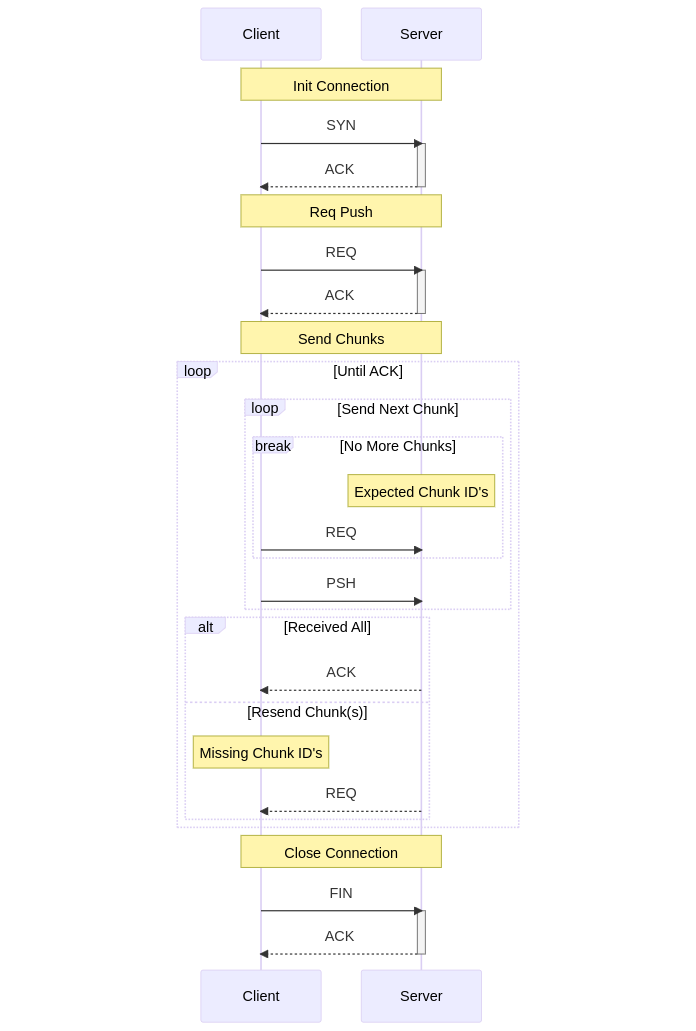
\includegraphics[width=0.9\linewidth]{p1-sequence.png}
    \caption{Prototype One Sequence Diagram}
    \label{fig:p1-sequence}
\end{figure}
\newpage

\subsection*{Testing}
After the initial tests several issues in the code needed to be fixed. These are listed below (with git commit hashes):

\begin{itemize}
    \item (1e67ab) payload offset out by 1, causing payload to be incorrectly stored
    \item (dfb553) message size prediction code miss-calculates header + meta length fields, causing header and meta fields sizes to be incorrect; creating an invalid packet
    \item (35db84) client starting chunk id is 0, should be 1
    \item (455708) buffer payload was not copied (instead referenced), causing next request to alter payload values
\end{itemize}

After testing prototype one it has been found that the overhead in transferring a single file is less than the existing protocols having only "0.14\%" overhead; shown in Table~\ref{tab:prototypes-test-results}. It also sent out less packets than the existing solutions, only "39".

When testing with text files the prototype produced "7.48\%" of overhead, comparing this to the best performing existing protocol rsync which was less "5.64\%". Whilst rsync is less it is only a
"1.84\%" more, this could likely be reduced further in a future prototype.

In the next test with a collection of photos; the prototype produced a higher overhead compared to all investigated existing solutions "1.73\%", however the number of packets sent is lower "1,128". This likely points to the individual packets for transferring the physical file data having more overhead. If this was the final solution, it would be ineffective for transferring larger files since the amount of wasted data would scale with the file size.

In the last test which used a purely synthetic scenario; sending many small files sized at 1KB. The prototype produced a overhead of "~18\%" extra compared to rsync which was the best performing existing solution. Compared to the photos test, this scenario shows that this prototype has a greater amount of overhead sent for negotiating a file before transfer. However this overhead may be acceptable as rsync provides little safeguarding around file locking, compared to this prototype which if fully completed would issue an error packet before allowing a transfer to occur. Compared to the other protocols which do implement file locks (FTP and SMB2); this prototype has a smaller overhead. Looking at the number of packets sent; shows that "2,504" were sent, comparing this to rsync only "69" were sent. This is a very large difference. This prototype can only send chunks relating to the current file until the next is negotiated, whereas in rsync multiple files can be included in a single packet, making it more suitable for transferring small files, when many can fit in a single packet. Reducing the number of packets sent over the network can reduce both latency and the amount of traffic transferred allowing the bandwidth to be repurposed for another task.

This test measured a "8.0Gbps" in transfer speed. Whilst that may seem very high it is due to UDP (and the prototype) not requiring acknowledgements for each packet.

During testing it has been discovered that when many file chunks during a large transfer are lost, it will only be until the end of the transfer before they can be re-sent. This is not ideal, since on a higher latency network it could be quite a long time before the end of a transfer; resulting in a longer total transfer time. This could be improved by sending the chunks in blocks, for example 20 chunk packets could be sent then verified until either missing ones are re-sent or a new block is started. This would allow for a smaller amount of chunks to be required to be re-sent during a large transfer.

It has also been found that having two serialized fields (header, metadata) is also not ideal, since multiple complex steps have to be taken until the message can be handled. First the packet type has to be inspected, then the header must be deserialized before the metadata can be processed. This could be reduced to where only a packet type and header is sent, this would also reduce the amount of reserved space in a packet for the metadata length field; which takes up 8 bytes.
